\documentclass{article}

\usepackage{ctex}
\usepackage{tikz}
\usetikzlibrary{calc}
\usetikzlibrary{cd}
\usetikzlibrary{decorations.pathreplacing}

\usepackage{amsthm}
\usepackage{amsmath}
\usepackage{amssymb}

\usepackage{pgfplots}
\pgfplotsset{compat=newest}

\usepackage{hyperref} %url
\hypersetup{
    colorlinks=true,
    linkcolor=blue,
    filecolor=magenta,      
    urlcolor=cyan,
    pdftitle={Overleaf Example},
    pdfpagemode=FullScreen,
    }

\usepackage{enumitem}

\usepackage[textwidth=18cm]{geometry} % 设置页宽=18

\usepackage{blindtext}
\usepackage{bm}
\parindent=0pt
\setlength{\parindent}{2em} 
\usepackage{indentfirst}


\usepackage{xcolor}
\usepackage{titlesec}
\titleformat{\section}[block]{\color{blue}\Large\bfseries\filcenter}{}{1em}{}
\titleformat{\subsection}[hang]{\color{red}\Large\bfseries}{}{0em}{}
%\setcounter{secnumdepth}{1} %section 序号

\newtheorem{theorem}{Theorem}[section]
\newtheorem{lemma}[theorem]{Lemma}
\newtheorem{corollary}[theorem]{Corollary}
\newtheorem{proposition}[theorem]{Proposition}
\newtheorem{example}[theorem]{Example}
\newtheorem{definition}[theorem]{Definition}
\newtheorem{remark}[theorem]{Remark}
\newtheorem{exercise}{Exercise}[section]
\newtheorem{annotation}[theorem]{Annotation}

\newcommand*{\xfunc}[4]{{#2}\colon{#3}{#1}{#4}}
\newcommand*{\func}[3]{\xfunc{\to}{#1}{#2}{#3}}

\newcommand\Set[2]{\{\,#1\mid#2\,\}} %集合
\newcommand\SET[2]{\Set{#1}{\text{#2}}} %

\newcommand{\norm}[1]{\left\lVert#1\right\rVert} % 范数
\newcommand{\vect}[1]{\mathbf{#1}} % vector
\newcommand{\hints}{{\color{blue} \text{hints}}}

\DeclareMathOperator{\arcsec}{arcsec}%反三角函数
\DeclareMathOperator{\arccot}{arccot}
\DeclareMathOperator{\arccsc}{arccsc}

\newcommand{\redt}[1]{\textcolor{red}{#1}}
\newcommand{\bluet}[1]{\textcolor{blue}{#1}}

\begin{document}
\title{考研高数习题集}
\author{枫聆}
\maketitle
\tableofcontents


\newpage
\section{极限相关}

\subsection{$1^\infty$类型极限}

\begin{example}
若$\lim \alpha(x)=0,\lim \beta(x)=\infty$,且$\lim \alpha(x)\beta(x) = A$,其中$A$是一个常数,则
$$
\lim \left[ 1 + \alpha(x) \right]^{\beta(x)} = e^A.
$$
\hints\ 带指数形式的表达式,第一想法是把指数拿下来
$$
\lim \left[ 1 + \alpha(x) \right]^{\beta(x)} = \lim e^{\beta(x)\ln(1+\alpha(x))} = \lim e^{\beta(x)\alpha(x)} = e^A.
$$
\end{example}

\begin{example}
求极限
$$
\lim\limits_{x \rightarrow \infty} \left[ \frac{x^2}{(x-a)(x+b)}\right]^x.
$$
\hints
$$
\left[ \frac{x^2}{(x-a)(x+b)}\right]^x = \left(\frac{x}{x-a}\right)^x \cdot \left(\frac{x}{x+b} \right)^x = \left(1+\frac{a}{x-a}\right)^x \cdot \left(1-\frac{b}{x+b}\right)^x = e^{a-b}.
$$
\end{example}

\begin{example}
求极限
$$
\lim\limits_{n \rightarrow \infty} \left( \frac{\sqrt[n]{a} + \sqrt[n]{b} + \sqrt[n]{c}}{3} \right)^n.
$$
\hints\ 往$(1+\alpha(x))^{\beta(x)}$上凑
$$
\left( \frac{\sqrt[n]{a} + \sqrt[n]{b} + \sqrt[n]{c}}{3} \right)^n = \left( 1 + \frac{\sqrt[n]{a} + \sqrt[n]{b} + \sqrt[n]{c}-3}{3}\right)^n
$$
考虑$\alpha(x)\beta(x)$
$$
\frac{(\sqrt[n]{a}-1) + (\sqrt[n]{b}-1) + (\sqrt[n]{c}-1)}{3}\cdot n = \frac{1}{3}\left( \frac{\sqrt[n]{a}-1}{\frac{1}{n}} + \frac{\sqrt[n]{b}-1}{\frac{1}{n}} + \frac{\sqrt[n]{c}-1}{\frac{1}{n}}\right)
$$
\end{example}

\subsection{$1^0$类型极限}

\begin{example}
\rm 若$\lim \alpha(x) = 0, \lim \beta(x)\alpha(x) = 0$,则
$$
(1+\alpha(x))^{\beta(x)} - 1 \sim \alpha(x)\beta(x).
$$
\hints\ 取对数
$$
e^{\beta(x)\ln(1+\alpha(x))}-1 \sim e^{\beta(x)\alpha(x)} -1 \sim \beta(x)\alpha(x). 
$$ 

\end{example}


\newpage
\subsection{夹逼准则应用}

\begin{example}
求极限
$$
\lim\limits_{n \rightarrow \infty}\left( \frac{n}{n^2+1} + \frac{n}{n^2+2} + \cdots + \frac{n}{n^2+n} \right).
$$
\hints
$$
\frac{n^2}{n^2+n} \leq s \leq  \frac{n^2}{n^2+1}.
$$
\end{example}

\begin{example}
求极限
$$
\lim\limits_{n \rightarrow 0^+} x\left[ \frac{1}{x} \right].
$$
\hints
$$
x-1 \leq \left[ x \right] \leq x
$$
\end{example}

\begin{example}\label{motonone-sequence-1}
求极限
$$
\lim\limits_{n \rightarrow \infty} \frac{2^n}{n!}.
$$
\hints
$$
\left(\frac{2}{1}\right)\times\frac{2}{2}\times\frac{2}{3}\times \cdots \times \frac{2}{n}.
$$
\end{example}


\newpage
\subsection{级数相关的极限}

\begin{example} \label{ex:jishu1}
当$\lim\limits_{n \rightarrow \infty} a_n = A$,则
$$
\lim\limits_{n \rightarrow \infty} \frac{a_1+a_2+\cdots+a_n}{n} = A.
$$
\hints\ 直接考察
$$
\left|\frac{a_1+a_2+\cdots+a_n}{n} - A \right| = \left| \frac{(a_1-A)+(a_2-A)+\cdots+(a_n-A)}{n} \right|
$$
{\color{blue}用极限的定义等式右边分成两部分},即对任意的$\varepsilon > 0$,可以找到一个$n_1$,使得$n > n_1$时有$|x_n - A| < \varepsilon$,那么
$$
\begin{array}{ll}
\left|\frac{(a_1-A) + (a_2-A) + \cdots + (a_{n_1}-A)}{n} + \frac{(a_{n_1 + 1}-A)+ (a_{n_1 + 2}-A) + \cdots + (a_{n}-A)}{n} \right| \\ \leq \frac{|a_1-A| + |a_2-A| + \cdots + |a_{n_1}-A|}{n} + \frac{|a_{n_1 + 2}-A|+ |a_{n_1 + 1}-A| + \cdots + |a_{n}-A|}{n}
\end{array}
$$
上述不等式右边第一项,形如$\frac{C}{n}$,因为先对任意$n > n_1$都有上述不等式成立,那么只需要让$n$取的大一点,就能使得$\frac{C}{n} < \varepsilon$({\color{red}阿基米德公理}). 右边第二项显然小于$\frac{n-n_1}{n}\varepsilon$,于是综上
$$
\left|\frac{a_1+a_2+\cdots+a_n}{n} - A \right| < \varepsilon+\frac{n-n_1}{n}\varepsilon < 2\varepsilon.
$$
{\color{blue}如果题目中没有直接给出极限的具体值,我们可以用O.Stolz定理先猜出来,然后用初等方法来验证,再根据极限的唯一性,就得到了答案}. 把$a_n$换成形式,例如
$$
\lim\limits_{n \rightarrow \infty} \frac{1+\sqrt[2]{2}+\cdots+\sqrt[n]{n}}{n} = \lim\limits_{n \rightarrow \infty} \sqrt[n]{n} = 1.
$$ 
\end{example}


\begin{example}
求极限
$$
x_n  = \frac{1^k + 2^k + \cdots + n^k}{n^{k+1}}.
$$
\hints\ 用O.Stolz定理考虑
$$
\lim\limits_{n \rightarrow \infty} \frac{n^k}{n^{k+1} - (n-1)^{k+1}}
$$
分母二项式展开合并极有$\lim \frac{n^k}{(k+1)n^k + \cdots} = \frac{1}{k+1}$. 这道题初等方法似乎不能很好的把握,用和式的方法写出来其实就是黎曼积分的定义
$$
\lim\limits_{n \rightarrow \infty} \frac{1}{n} \sum\limits_{k=1}^k \frac{k}{n} = \int_0^1 x^k = \frac{1}{k+1}. 
$$
{\color{blue} 级数相关的问题往往可以尝试考虑用定积分的思路来解决}. 下面是$1^k + 2^k +\cdots + n^k$的转换思路
$$
{\color{red}
\sum_{i=1}^n i^k=n^{k+1}\frac1n\sum_{i=1}^n \left(\frac in\right)^k\sim_\infty n^{k+1}\int_0^1 x^kdx=\frac{n^{k+1}}{k+1}
}
$$
\end{example}

\newpage
\begin{example}\label{ex:jishu2}
当$\lim\limits_{n \rightarrow \infty} a_n = a, a_n > 0$,则
$$
\lim\limits_{n \rightarrow \infty } \ln \sqrt[n]{a_1a_2\cdots a_n} = \ln a.
$$
\hints\
$$
\ln \sqrt[n]{a_1a_2\cdots a_n} = \frac{\ln a_1 + \ln a_2 + \cdots + \ln a_n}{n} = \ln a.
$$
因为$\ln x$的连续性,所以$\lim \ln a_n = \ln a$,再根据\ref{ex:jishu1}. 
\end{example}

\begin{example}\label{ex:jishu3}
当$\lim\limits_{n \rightarrow \infty} a_n = a, a_n > 0$,则
$$
\lim\limits_{n \rightarrow \infty} \sqrt[n]{a_1a_2\cdots a_n} = a.
$$
\hints\ 取对数再根据\ref{ex:jishu2}
$$
\sqrt[n]{a_1a_2\cdots a_n} = e^{\ln \sqrt[n]{a_1a_2\cdots a_n}} = e^{ln a} = a.
$$
\end{example}

\begin{example}
求极限
$$
\lim\limits_{n \rightarrow \infty}\frac{\sqrt[n]{n!}}{n}.
$$
\hints\ 由 \ref{ex:jishu3} 可知$a_n$和$b_n = \sqrt[n]{a_1a_2\cdots a_n}$的极限是相同的(假设$a_n$的极限存在). 那么有一个推论,对于数列
$$
a_1, \frac{a_2}{a_1}, \frac{a_3}{a_2},\cdots,\frac{a_{n+1}}{a_n},\cdots
$$
则$\lim \sqrt[n]{a_n} = \lim \frac{a_{n+1}}{a_{n}}$,只要等式右边的极限存在就行. 在这里我们只要设$a_n = \frac{n!}{n^n}$即可,那么
$$
\lim \frac{(n+1)!}{(n+1)^{n+1}} \cdot \frac{n^n}{n!} = \lim \frac{n^n}{(n+1)^n} = \frac{1}{(1+\frac{1}{n})^n} = \frac{1}{e}.
$$
\end{example}

\newpage
\subsection{去除根式的尴尬}

%https://math.stackexchange.com/questions/3491441/limit-lim-limits-x-to-infty-sqrtnxa-1xa-2-xa-n-x?noredirect=1&lq=1
\begin{example}
求极限
$$
\lim\limits_{x \rightarrow +\infty} \left[ \sqrt[k]{(x+a_1)(x+a_2)\cdots(x+a_k)} - x\right].
$$
\hints\ 
$$
(x+a_1)(x+a_2)\cdots(x+a_k) = x^k\left(1+\frac{a_1+a_2+\cdots+a_k}{x}+\mathcal{O}\left(\frac{1}{x^2}\right)\right)
$$
那么
$$
x\left(1+\frac{a_1+a_2+\cdots+a_k}{x}+\mathcal{O}\left(\frac{1}{x^2}\right)\right)^{\frac{1}{n}} = x\left(1+ \frac{a_1+a_2+\cdots+a_n}{nx} + \mathcal{O}\left(\frac{1}{x^2}\right)\right) = x + \frac{a_1+a_2+\cdots+a_n}{nx} + \mathcal{O}\left(\frac{1}{x}\right),
$$
这里第一个等号右边对$(1+x)^p$在$x=0$处用了一下{\color{blue}泰勒展开}得到$(1+qx+\mathcal{O}(x^2))$,这个$\mathcal{O}$表示最高次的多项式. 

还有一种{\color{blue}升次}的方法,即下面的恒等式
$$
{\color{red}
y-z = \frac{y^k-z^k}{y^{k-1} + y^{k-2}z + \cdots + z^{k-1}}.
}
$$
这里我们使得$y = \sqrt[k]{(x+a_1)(x+a_2)\cdots(x+a_k)}$及$z = x$,那么原式就变成了
$$
\begin{array}{lll}
= &\frac{(x+a_1)(x+a_2)\cdots(x+a_k) - x^k}{\left[\sqrt[k]{(x+a_1)(x+a_2)\cdots(x+a_k)}\right]^{k-1}+\left[\sqrt[k]{(x+a_1)(x+a_2)\cdots(x+a_k)}\right]^{k-2}x + \cdots + x^{k-1} } \\
= & \frac{a_1+a_2+\cdots + a_k + \mathcal{O}(\frac{1}{x})}{\left[\sqrt[k]{(1+\frac{a_1}{x})(1+\frac{a_2}{x})\cdots(1+\frac{a_k}{x})}\right]^{k-1}+\left[\sqrt[k]{(1+\frac{a_1}{x})(1+\frac{a_2}{x})\cdots(1+\frac{a_k}{x})}\right]^{k-2}x + \cdots + 1} & {\color{blue}\text{上下除以$x^{k-1}$}}
\end{array}
$$
分母中$\sqrt[k]{(1+\frac{a_1}{x})(1+\frac{a_2}{x})\cdots(1+\frac{a_k}{x})}$是趋于$1$的,再用一下函数$x^{\frac{m}{n}}$的连续性,取其函数值也是等于$1$,所以分母就有$k \cdot 1$.
\end{example}

%https://math.stackexchange.com/questions/28348/proof-of-lim-n-to-infty-sqrtnn-1
\begin{example}
求极限
$$
\lim\limits_{n \rightarrow \infty} \sqrt[n]{n} = 1.
$$
\hints\ 取对数应用$e^x$的连续性
$$
\lim e^\frac{\ln n}{n} = e^{\lim \frac{\ln n}{n}} = 1. 
$$
也可以使用一下\ref{prop: bonuli}的伯努利不等式来证明,这里设$\sqrt[n]{n} = 1+h$,那么
$$
\begin{array}{ll}
&n = (1+h)^n = 1+nh + \frac{n(n-1)}{2}h^2 + \cdots \\
\Rightarrow & n \geq \frac{n(n-1)}{2}h^2  \\
\Rightarrow & h^2 \leq \frac{2}{n-1}.
\end{array}
$$
当$n \rightarrow \infty$时,$h \rightarrow 0$,即$\sqrt[n]{n}-1 \rightarrow 0$,所以$\lim \sqrt[n]{n} = 1$.
\end{example}

\begin{example}
\rm 求极限
$$
\lim\limits_{x\to +\infty} (\sqrt[6]{x^6 + x^5}-\sqrt[6]{x^6 - x^5})
$$
\hints\ 考虑把根式里面变成$(1+\alpha(x))$的形式,因此考虑提出一个因子$x$
$$
\lim\limits_{x\to +\infty} x(\sqrt[6]{1+\frac{1}{x}}-\sqrt[6]{1-\frac{1}{x}}) = \lim\limits_{x\to +\infty} \left(  \frac{\sqrt[6]{1+\frac{1}{x}}}{\frac{1}{x}} - \frac{\sqrt[6]{1-\frac{1}{x}}}{\frac{1}{x}} \right) = \frac{1}{3}.
$$
\end{example}

\newpage
\subsection{换元取极限}

\begin{example}
求极限
$$
\lim\limits_{x \rightarrow 0} \frac{\sqrt[m]{x+1}-1}{x},\; m \in \mathbb{N}.
$$
\hints\ 设$y = \sqrt[m]{x+1}-1$,显然$y$在$x = 0$处连续,所以当$x \rightarrow 0$时有$y \rightarrow 0$,那么此时的极限就变成了
$$
\lim\limits_{y \rightarrow 0} \frac{y}{(y+1)^m-1} = \frac{1}{m}.
$$
这样上下都变成我们熟悉的多项式,分母二项式展开.
\end{example}

\begin{example}
求极限
$$
\lim\limits_{x \rightarrow 0} \frac{(x+1)^{\frac{n}{m}}-1}{x}.
$$
\hints\ 还是使得$y = (x+1)^{\frac{1}{m}}-1$,那么就变成了
$$
\lim\limits_{y \rightarrow 0} \frac{(1+y)^n-1}{(1+y)^m-1} = \lim\limits_{y \rightarrow 0} \frac{(1+y)^n-1}{y}\frac{y}{(1+y)m-1} = \frac{n}{m}. 
$$
\end{example}

\subsection{递归求极限}

\begin{example}
\rm \ref{motonone-sequence-1} 单调数列求极限

\hints\ 考虑递归式
$$
x_{n+1} = x_n \cdot \frac{2}{n+1},
$$
等式两边同时取极限则有
$$
a = a \cdot 0 \Rightarrow a = 0. 
$$
\end{example}

\subsection{等价无穷小的替换}


\subsection{中值定理}

\begin{example}
\rm 求极限
$$
\lim\limits_{x \to +\infty} \frac{1}{2}x^2[\ln\arctan(x+1) - \ln\arctan x]. 
$$
\hints\ 对连续函数$\ln\arctan x$应用中值定理
$$
\lim\limits_{x \to +\infty} \frac{1}{2}x^2 \frac{1}{[1+(\theta+x)^2]\arctan (\theta+x)},
$$
其中$0 < \theta < 1$. 那么即有
$$
\lim\limits_{x \to +\infty} \frac{1}{2} \frac{x^2}{1+(\theta+x)^2} \frac{1}{\arctan (\theta+x)} = \frac{1}{\pi}.
$$
\end{example}

\begin{example}
\rm 求极限
$$
I = \lim\limits_{x \to 0}\frac{\cos(xe^x)-e^{-\frac{x^2}{2}e^{2x}}}{x^4}.
$$

\hints\ 这里设$xe^x = t$,则有
$$
I =  \lim\limits_{x \to 0}\frac{\cos(t)-e^{-t^2}}{t^4} \cdot e^{4x} = \lim\limits_{t \to 0}\frac{\cos(t)-e^{-\frac{t^2}{2}}}{t^4},
$$
这里用泰勒展开是比较好的,
$$
\begin{array}{ll}
\cos t = 1 - \frac{t^2}{2!} + \frac{t^4}{4!} + o(t^4)\\
e^{-\frac{t^2}{2}} = 1 + \frac{-\frac{t^2}{2}}{1!} + \frac{\frac{t^4}{4}}{2!}+o(t^4)
\end{array}
$$
因此
$$
I = \lim\limits_{t \to 0} \frac{\frac{t^4}{24}-\frac{t^4}{8}+o(t^4)}{t^4} = -\frac{1}{12}.
$$
\end{example}

\subsection{含积分的极限}

%https://math.stackexchange.com/questions/4228847/how-to-calculate-lim-x-to-0-frac-int-0x-sqrtx-tetdt-sqrtx3
\begin{example}
\rm 求极限
$$
\lim _{x\to 0^+} \frac{\int _0^x\sqrt{x-t}e^tdt}{\sqrt{x^3}}
$$
\hints\ 这样的含参数积分最好的办法就是洛必达,但是这里首先需要换元一下,令$u = x-t$,则
$$
\int _0^x\sqrt{x-t}e^tdt = \int_{0}^x \sqrt{u}e^{x-u}du = e^x \sqrt{u}e^{-u}du.
$$
再用洛必达
$$
\lim _{x\to 0^+} = \frac{e^x \sqrt{u}e^{-u}du}{x^{\frac{3}{2}}}  = \lim _{x\to 0^+} \frac{( \int_{0}^x \sqrt{u}e^{-u}du)'}{(x^{\frac{3}{2}})'} = \frac{x^{\frac{1}{2}}e^{-x}}{\frac{3}{2}x^{\frac{1}{2}}} = \frac{2}{3}.
$$
\end{example}

\subsection{没有具体的函数表达式}

\begin{example}
\rm 设$f(x)$在$x=a$处二阶导数存在,求
$$
L = \lim\limits_{h \to 0}\frac{\frac{f(a+h)-f(a)}{h}-f'(a)}{h}. 
$$
\hints\ 直觉告诉它的结果和二阶导有关,但是任何初等方法都化不出来二阶导的定义,这个时候可以考虑用一下洛必达
$$
L = \lim\limits_{h \to 0} \frac{f(a+h)-f(a)-hf'(a)}{h^2} = \lim\limits_{h \to 0} \frac{f'(a+h)-f'(a)}{2h} = \frac{1}{2}f''(a). 
$$
\end{example}

\subsection{三角函数相关}

\begin{example}
\rm 求
$$
\lim\limits_{n \to \infty} \sin^2(\pi \sqrt{n^2+n}). 
$$

\hints\ 这个积分有点反直觉,主要是变量放在了$\sin$里面. 
$$
\lim\limits_{n \to \infty} \sin^2(\pi \sqrt{n^2+n}) = \lim\limits_{n \to \infty} \sin^2[\pi(\sqrt{n^2 + n} -n)] = \lim\limits_{n \to \infty} \sin^2\left(\pi \frac{n}{\sqrt{n^2+n}+n} \right) = \sin^2 \frac{\pi}{2} = 1. 
$$

再来搞点不是那么反直觉的东西,
$$
\lim\limits_{n \to \infty} \sin^2 \left(\pi n \sqrt{1+\frac{1}{n}} \right),
$$
这里可以尝试将$\sqrt{1+\frac{1}{x}}$展开,首先
$$
\sqrt{1+x} = 1  + \frac{x}{2}+o(x),
$$
于是
$$
\sqrt{1+\frac{1}{x}} = 1 + \frac{1}{2}\cdot\frac{1}{x} + o(\frac{1}{x})
$$
因此
$$
\lim\limits_{n \to \infty} \sin^2 \left(\pi n (1 + \frac{1}{2}\cdot\frac{1}{n}+o(\frac{1}{n})) \right) = \sin^2\frac{\pi}{2}
$$
\end{example}

\begin{example}
\rm 求极限
$$
\lim\limits_{x \to 0} \frac{\cos(\sin x)-\cos x}{(1-\cos x)\sin^2 x}
$$
\hints\ 方法1: 直接泰勒爆算即可,其中
$$
\cos(\sin x) = 1 - \frac{\sin^2}{2!} + \frac{\sin^4}{4!} + o(\sin^4). 
$$
再把$\sin ^x = x -\frac{x^3}{3!} + o(x^3)$带入,
$$
\cos(\sin x) = 1 - \frac{(x -\frac{x^3}{3!} + o(x^3))^2}{2!} + \frac{(x -\frac{x^3}{3!} + o(x^3))^4}{4!} + o(x^4),
$$
这里泰勒余项要把握好,因为分母等价无穷小为$\frac{x^4}{2}$. 整理一下即有
$$
\cos(\sin x) = 1-\frac{x^2}{2!} + (\frac{1}{3!}+\frac{1}{4!})x^4 + o(x^4),
$$

方法2: 对分子用和差化积简化直接泰勒的压力,即
$$
\cos(\sin x)-\cos x = \cos\left( \frac{\sin x+x}{2} + \frac{\sin x-x}{2} \right) - \cos\left( \frac{\sin x+x}{2} - \frac{\sin x-x}{2} \right),
$$
于是
$$
\cos(\sin x)-\cos x  = -2\sin\left( \frac{\sin x+x}{2}  \right)\sin\left( \frac{\sin x-x}{2}\right) \sim \frac{(\sin x+x)(x-\sin x)}{2},
$$
因此
$$
\lim\limits_{x \to 0} \frac{\cos(\sin x)-\cos x}{(1-\cos x)\sin^2 x} = \lim\limits_{x \to 0} \frac{x^2 - \sin^2}{x^4} =  \lim\limits_{x \to 0} \frac{x^2-(x-\frac{x^3}{3}+o(x^3))^2}{x^4} = \lim\limits_{x \to 0} \frac{\frac{2}{3!}x^4 + o(x^4)}{x^4} = \frac{1}{3}.
$$
\end{example}


\subsection{极限存在性}

\begin{annotation}
\rm \redt{左极限和右极限是否存在且相等}. 
\end{annotation}

\begin{example}
\rm 求下述函数$x \to 1$时的极限是否存在
$$
f(x) = \frac{\sin \pi x}{x-1}e^{\frac{1}{(x-1)^3}}. 
$$
\hints\ 其中
$$
\lim\limits_{x \to 1} \frac{\sin \pi x}{x-1} = \lim\limits_{x \to 1} \frac{-\sin(\pi(x-1))}{x-1} = -\pi, 
$$
而
$$
\lim\limits_{x \to 1^+} e^{\frac{1}{(x-1)^3}} = +\infty, \lim\limits_{x \to 1^-} e^{\frac{1}{(x-1)^3}} = 0,
$$
因此$\lim\limits_{x \to 1} f(x)$不存在. 
\end{example}

\newpage
\section{导数}

\subsection{导数定义相关的}

\begin{example}
\rm 已知$f'(x_0) = -1$,求
$$
\lim\limits_{x \to 0} \frac{x}{f(x_0-2x)-f(x_0-x)}.
$$
\hints 直觉上就是想办法凑导数的定义出来
$$
\begin{array}{ll}
\lim\limits_{x \to 0} \frac{f(x_0-2x)-f(x_0)}{-2x} = -1 \\
\lim\limits_{x \to 0} \frac{f(x_0-x)-f(x_0)}{-x} = -1\\
\end{array}
$$
求出需要$\lim\limits_{x \to 0} \frac{f(x_0-2x)-f(x_0)}{x}$和$\lim\limits_{x \to 0} \frac{f(x_0-x)-f(x_0)}{x}$,两项相减再取倒. 
\end{example}

\subsection{泰勒公式求高阶导数}

\subsection{递归法求高阶导数}

%通项推导 https://math.stackexchange.com/questions/549028/deriving-maclaurin-series-for-frac-arcsin-x-sqrt1-x2
\begin{example}
\rm 设
$$
f(x) = \frac{\arcsin x}{\sqrt{1-x^2}},
$$
求$f^{(n)}(0)$.

\hints\ 这道题你想求它的麦克劳林级数其实不太好求(\url{https://math.stackexchange.com/questions/549028/deriving-maclaurin-series-for-frac-arcsin-x-sqrt1-x2}),实际上也不用求出通项,因为只需要求$x=0$的情况,这里有比较trick的利用递归式的手法. 先求它的一阶导
$$
f'(x) = \frac{1 + \frac{x}{\sqrt{1-x^2}}\arcsin x}{1-x^2} = \frac{x}{(1-x)^{3/2}}\arcsin x + \frac{1}{1-x^2}.  
$$
这里构造一个微分方程
$$
(1-x^2)f'(x)-xf(x)-1 = 0
$$ 
两边求$n$次,根据$n$的莱布尼茨公式有
$$
(1-x^2)f^{(n+1)}(x) - (2n+1)xf^{n}(x)-n^2f^{(n-1)}(x) = 0. 
$$
带入$x=0$,这里就可能消掉$f^{(n)}$的项,得到一个递归式
$$
f^{(n+1)}(0) - n^2f^{(n-1)}(0). 
$$
这里我们让$n=n+1$,则有
$$
f^{(n+2)}(0) =  n^2f^{(n)}(0). 
$$
我们可以求出最前面的两项$f'(0) = 1$和$f''(0) = 0$, 于是这里有
$$
f^{n}(0) = \left\{ \begin{array}{ll}
0 & n=\text{奇数} \\
(n-1)^2\times(n-2)!\times\cdots\times 2! &   n=\text{偶数}
\end{array} \right.
$$
奇数下的情况可以化简为$2^{n-1}((\frac{n-1}{2})!)^2$
\end{example}

\newpage
\section{函数性质}

\subsection{求零点}

\begin{example}
\rm 设$f(x)$在$[a,b]$可导,$f'_+(a) > 0, f'_-(b) > 0, f(a) \geq f(b)$. 则$f'(x)$在$[a,b]$上有两个零点. 

\hints\ $f'(x)$有两个零点,也就是有两个极值点. 这样的题目最好还是构造相应的函数,用罗尔定理来做. 设$g(x) = f(x)-f(a)$和$h(x)=f(x)-f(b)$,我们思路是确定$g(x)$和$h(x)$的一个零点,那么就可以用罗尔定理来确定两个$f'(x)$的零点. 确定$g(x)$和$h(x)$零点,我们要用零点定理来做. 由于$f'_+(a) > 0$,根据导数的定义有
$$
\lim\limits_{x \to 0^+} \frac{f(a+x)-f(a)}{x} > 0 \Rightarrow f(a + \xi_1) > f(a),\xi_1 > 0
$$  
同理,由于$f'_-(b) > 0$,我们可以得到
$$
\lim\limits_{x \to 0^+} \frac{f(b-x)-f(b)}{-x} > 0 \Rightarrow f(b - \xi_2) < f(b), \xi_2 > 0.
$$
注意这里的$\Rightarrow$用到的是极限的保号性. 于是这里由零点定理有
$$
g(a + \xi_1) > 0, g(b-\xi_1) \leq 0 \Rightarrow g(\theta_1) = 0, \,a+\xi_1 < \theta_1 < b-\xi_1
$$
因此存在$f(\theta_1) = f(a)$. 同理有
$$
h(a+\xi_1) > 0, h(b-\xi_2) < 0 \Rightarrow g(\theta_2) = 0, \,a+\xi_1 < \theta_2 < b-\xi_1
$$
因此存在$f(\theta_2) = f(b)$.  

现在需要分类讨论一下,若$\theta_1  \leq \theta_2$,则根据罗尔定理我们可以在$(a,\theta_1)$及$(\theta_2,b)$上各找到一个零点. 若$\theta_1 > \theta_2$,此时由$g(a+\xi_1) > 0, g(\theta_2) \leq 0$,存在一点$\theta_3$使得$f(\theta_3) = 0$,同理由$g(\theta_1) \geq 0, g(b-\xi_2) < 0$,可以找到一点$\theta_4$使得$f(\theta_4) = 0$,这样$\theta_3 < \theta_4$,回到了前面一种情况. 证闭!


\end{example}


\newpage
\section{不定积分}

\subsection{多项式分式}

\begin{example}
\rm 求
$$
\int \frac{x^4-x^2}{1+x^2}dx.
$$
\hints\ 还是得部分分式
$$
\frac{x^4-x^2}{1+x^2} = \frac{(x^4-1) -(x^2+1) + 2 }{1+x^2}
= x^2 + \frac{2}{1+x^2}-2.
$$
因此原函数为
$$
\frac{x^3}{3} + 2\arctan x - 2x + C,
$$ 
\end{example}

\begin{example}
\rm 求
$$
\int \frac{x+5}{x^2-6x+13}dx.
$$
\hints 观察分子多项式次数小于分母的,且只小一次,所以我们考虑这样部分分式
$$
\frac{1}{2}\int \frac{2x-6}{x^2-6x+13}dx + 8\int \frac{1}{x^2-6x+13}dx = \frac{1}{2}\int \frac{1}{x^2-6x+13}d(x^2-6x+13) + 8\int \frac{1}{4+(x-3)^2}dx,
$$
因此原函数为
$$
\frac{1}{2}\ln(x^2-6x+13) +  4\arctan \frac{x-3}{2} +C.
$$
\end{example}

\begin{example}
\rm 求
$$
\int \frac{x}{x^4+2x^2+5}dx 
$$
\hints\ 观察分子多项式次数小于分母,且小两次,所以我们考虑这样部分分式
$$
\int \frac{x}{4+(x^2+1)^2}dx = \frac{1}{2}\int \frac{1}{4+(x^2+1)^2}d(x^2+1) = \frac{1}{4}\arctan \frac{x^2+1}{2} + C
$$
\end{example}

\subsection{分母带根号}

\begin{example}
\rm 求
$$
\int \frac{dx}{\sqrt{x(4-x)}}.
$$
\hints 根号下凑平方
$$
\int \frac{1}{\sqrt{4-(x-2)^2}}d(x-2) = \arcsin \frac{x-2}{2} +C
$$
\end{example}

\begin{example}
\rm 求
$$
\int \frac{2-x}{\sqrt{3+2x-x^2}}dx.
$$
\hints\ 先分式把分子根号里面的微分
$$
\int \frac{2-x}{\sqrt{3+2x-x^2}}dx = \int \frac{1-x}{\sqrt{3+2x-x^2}} dx + \int \frac{1}{\sqrt{3+2x-x^2}} dx = \frac{1}{2}\int \frac{1}{\sqrt{3+2x-x^2}} d(3+2x-x^2) +  \int \frac{1}{\sqrt{4-(x-1)^2}} dx,
$$
因此原函数为
$$
\sqrt{3+2x-x^2} + \arcsin \frac{x-1}{2} + C
$$
\end{example}

\begin{example}
\rm 求
$$
\int \frac{x^2}{\sqrt{a^2 - x^2}}dx 
$$
\hints\ 考虑第二类换元,令$x=a\sin t$,则
$$
\int \frac{a^2\sin^2 t}{a\cos t} \cdot a\cos t dt = \frac{a^2}{2}\int 1-\cos 2t dt = \frac{a^2 t}{2} - \frac{a^2}{4}\sin 2t.
$$
把$t$变成$x$也有一点技巧,第二项可以变成$\frac{1}{2}(a\sin t)(a \cos t)$,其中$a\sin t = x, a\cos t = \sqrt{a^2 - x^2}$,这样会方便一点
$$
\frac{a^2\arcsin \frac{x}{a}}{2} - \frac{x}{2}\sqrt{a^2 - x^2}+C
$$
\end{example}

\begin{example}
\rm 求
$$
\frac{dx}{x\sqrt{x^4+1}}.
$$
\hints 这里还是要凑根号下的微分,有比较多的凑法,这里提及一种凑微分再配合三角换元的,
$$
\frac{dx}{x\sqrt{x^4+1}} = \int \frac{1}{2} \frac{dx^2}{x^2 \sqrt{(x^2)^2 + 1}},
$$
令$x^2 = \tan u$, 于是得到
$$
\frac{1}{2}\int \frac{1}{\sin u}du = \frac{1}{2} \ln |\csc u + \cot u|. 
$$
再带回$x$即可. 
\end{example}

\begin{example}
\rm 求
$$
\int \frac{dx}{\sqrt{1+x^2}(1+x^2)}.
$$
\hints\ 这里目标肯定是换元换成我们熟悉的积分,但是找不到因子提到微分符号里面,这时可以分母提一个$x^3$出来,就可以换元了
$$
\int \frac{dx}{x^3\sqrt{1+\frac{1}{x^2}}(1+\frac{1}{x^2})} = -\frac{1}{2} \int \frac{d(1+\frac{1}{x^2})}{\sqrt{1+\frac{1}{x^2}}(1+\frac{1}{x^2})} = \frac{1}{\sqrt{1+\frac{1}{x^2}}} + C
$$
这里也可以尝试令$x=\frac{1}{t}$,有
$$
-\int \frac{tdt}{\sqrt{1+t^2}(1+t^2)} = \int \frac{d\sqrt{1+x^2}}{1+x^2}
$$
\end{example}

\subsection{换元法}

\begin{example}
\rm 求
$$
\int \sqrt{1+e^x} dx
$$
\hints 考虑第二类换元,令$x = \ln (t^2-1)$,则
$$
\int t \cdot \frac{2t}{t^2-1} dt = 2 \int 1 + \frac{1}{t^2-1}dt =2t + \ln |\frac{t-1}{t+1}| + C
$$
带入$t=\sqrt{e^x +1}$,即得
$$
2\sqrt{e^x +1} + \ln \frac{\sqrt{e^x +1}-1}{\sqrt{e^x +1}+1} +C
$$
\end{example}

\subsection{高次}


\subsection{分部积分}

\subsection{三角有理式}

\begin{example}
\rm 求
$$
\int \frac{dx}{\cos x(1+\sin x)}.
$$
\hints\ 这里有一个非常巧妙的第二类换元,令$x=\arcsin u$,则
$$
\int \frac{1}{\sqrt{1-u^2}(1+u)} \frac{1}{\sqrt{1-u^2}}du = \int \frac{1}{(1+u)(1-u^2)}du .
$$
再把有理式拆开,这过程使用待定系数的方法
$$
\int \frac{1}{(1+u)(1-u^2)}du = \frac{1}{2}\int \frac{1}{1-u^2} + \frac{1}{(1+u)^2}du  = -\frac{1}{4} \ln \left| \frac{1-u}{1+u} \right| -\frac{1}{2}\frac{1}{(1+u)}. 
$$
最后即有
$$
-\frac{1}{4} \ln \left|\frac{1-\sin x}{1+\sin x}\right| - \frac{1}{2}\frac{1}{1+\sin x}+C. 
$$
\end{example}

\begin{example}
\rm 求
$$
\int \frac{dx}{\sin x(\sin x + \cos x)}.
$$
\hints\ 考虑第二类换元,令$x = \arccot u$,则有
$$
- \int \frac{1}{\frac{1}{\sqrt{1+u^2}}(\frac{1}{\sqrt{1+u^2}} + \frac{u}{\sqrt{1+u^2}})} \frac{1}{1+u^2} du = - \int \frac{1}{1+u}du = - \ln |u| + C = -\ln|1+\cot x| + C .
$$
\end{example}

\begin{example}
\rm 求
$$
\int \frac{\sin x}{\sin x + \cos x}dx
$$
\hints\ 这种情况可以考虑先化简一下分子,即上下乘以$(\cos x - \sin x)$,这样之后就可以考虑部分分式. 
\end{example}

\subsection{递归式}

\begin{example}
\rm 求
$$
\int e^{ax}\cos nx dx.
$$
\hints 分部积分2次回到原积分
$$
\begin{array}{ll}
\int e^{ax}\cos nx dx = \frac{1}{a}\int \cos nx d e^{ax}  &= \frac{1}{a}\left(e^{ax}\cos nx + n \int e^{ax}\sin nx dx \right) \\
&= \frac{1}{a}\left[ e^{ax}\cos nx + \frac{n}{a} \left( e^{ax}\sin nx - n\int e^{ax}\cos nxdx \right) \right]
\end{array}
$$
整理两边即得
$$
\frac{n^2 + a^2}{a^2} \int e^{ax}\cos nx dx = \frac{ae^{ax}\cos nx + ne^{ax}\sin nx}{a^2} \Rightarrow \int e^{ax}\cos nx dx = \frac{ae^{ax}\cos nx + ne^{ax}\sin nx}{a^2+n^2}
$$
类似的有
$$
\int e^{ax}\sin nx dx = \frac{ae^{ax}\sin nx - ne^{ax}\cos nx}{a^2+n^2}
$$
\end{example}


\subsection{被积函数含不常见函数形式}

\begin{example}
\rm 求
$$
\int \frac{\arcsin e^x}{e^x}dx. 
$$
\hints\ 必须得想办法吧$\arcsin e^x$提出来,因为我们没有已知原函数导数为反三角的,这里自然地就要使用部分积分了
$$
-\int \arcsin e^x d(e^{-x}) = -\frac{\arcsin e^x}{e^x} + \int e^{-x} \frac{e^x}{\sqrt{1-e^{2x}}}dx = \int \frac{1}{\sqrt{1-e^{2x}}}dx . 
$$
这里令$t=\sqrt{1-e^{2x}}$,那么$x = \frac{\ln(1-t^2)}{2},dx = \frac{-t}{1-t^2}dt$,于是
$$
\int \frac{1}{t} \frac{-t}{1-t^2}dt = \int\frac{1}{t^2-1}dt =  \frac{1}{2}\ln \left| \frac{t-1}{t+1} \right| + C = \frac{1}{2}\ln  \frac{\sqrt{1-e^{2x}}-1}{\sqrt{1-e^{2x}}+1}  + C.  
$$
因此
$$
\int \frac{\arcsin e^x}{e^x}dx = -\frac{\arcsin e^x}{e^x} + \frac{1}{2}\ln  \frac{\sqrt{1-e^{2x}}-1}{\sqrt{1-e^{2x}}+1}  + C  
$$
\end{example}

\begin{example}
\rm 求
$$
\int \ln\left( 1+\sqrt{\frac{1+x}{x}} \right)dx, x>0
$$
\hints 首选分部积分,但是为了为了能部分积分,我们必须先第一类换元,令$t = \sqrt{\frac{1+x}{x}}$,那么$x =\frac{1}{t^2-1}$,于是
$$
\int \ln(1+t)d\left(\frac{1}{t^2-1}\right) = \frac{\ln(1+t)}{{t^2-1}}- \int \frac{1}{(1+t)^2(t-1)},
$$
其中
$$
\int \frac{1}{(1+t)^2(t-1)} = \frac{1}{2}\int \frac{(t+1)-(t-1)}{(1+t)^2(t-1)} = \frac{1}{2} \int \frac{1}{t^2-1} - \frac{1}{(1+t)^2} = \frac{1}{4}\ln\left|\frac{t-1}{t+1} \right| + \frac{1}{2(1+t)} + C. 
$$
因此
$$
\int \ln\left( 1+\sqrt{\frac{1+x}{x}} \right)dx = \frac{\ln(1+t)}{{t^2-1}} + \frac{1}{4}\ln\left|\frac{t-1}{t+1} \right| + \frac{1}{2(1+t)} + C. 
$$
\end{example}

\newpage
\section{定积分}



\subsection{参数积分求导}

\begin{example}
\rm 设$f(x)$连续,求
$$
\frac{d}{dx}\int_0^x tf(x^2-t^2)dt.
$$
\hints\ 对于这种第二类的参数积分,对于有比较简洁的结果的,首先应该换元试试,令$u = x^2 - t^2$,那么即有
$$
-\frac{1}{2}\int_{x^2}^{0} f(u)du = \frac{1}{2}\int_{0}^{x^2} f(u)du 
$$
因此
$$
\frac{1}{2}\frac{d}{dx}\int_{0}^{x^2} f(u)du = xf(x^2). 
$$
\end{example}

\subsection{奇怪的定积分}

\begin{example}
\rm 设$f(x)=\int_0^{\pi} \frac{\sin t}{\pi-t}dt$,求$\int_0^{\pi}f(x)dx$.

\hints\ 可以用分部积分
$$
\int_0^{\pi}f(x)dx =  xf(x)\big\vert_0^{\pi} - \int_{0}^{\pi} xf'(x)dx =  \pi\int_{0}^{\pi} \frac{\sin x}{\pi-x}dx - \int_{0}^{\pi} \frac{\sin x}{\pi-x}dx = \int_{0}^{\pi} \sin x dx = 2. 
$$
\end{example}

\subsection{不太好积的带三角函数的积分}

\begin{example}
\rm 求
$$
I = \int_0^{\pi} \frac{x\sin x}{1+\cos^2 x}.
$$
\hints\ 如果不能一眼看出来
$$
I =  - \int_0^{\pi} x d\arctan\cos x = -\left. x\arctan\cos x\right|_0^\pi  + \int_0^{\pi} \arctan\cos x.  
$$
后面这个积分,令$u = \pi - x$,则可以得到
$$
\int_0^{\pi} \arctan\cos x = -\int_0^{\pi} \arctan\cos x,
$$
即它是等于零的. 

\redt{尝试方法} 我们要充分利用三角函数的性质,一开始我们令$u = \pi-x $,则有
$$
I = \int_0^\pi \frac{(\pi-u)\sin u}{1+\cos^u} \rightarrow 2I = \pi \int_0^{\pi} \frac{\sin x}{1+\cos^2x}dx = -\pi \left. \arctan\cos x\right|_0^\pi  = \frac{\pi^2}{2}
$$
\end{example}

\subsection{待定系数收敛反常积分}

\begin{example}
\rm 求满足下式的$a,b$
$$
\int_1^{+\infty} \left[ \frac{2x^2 + bx + a}{x(2x+a)} - 1\right]dx = 1
$$
\hints\ 首先化简一下
$$
\int_1^{+\infty} \frac{(b-a)x+a}{2x^2 + ax} dx
$$
若上述积分收敛,则$b=a$. 于是
$$
\int_1^{+\infty} \frac{a}{2x^2 + ax} dx = \int_1^{+\infty} \frac{1}{x} - \frac{2}{2x+a}dx = \left. \ln \frac{x}{2x+a} \right|_1^{+\infty} = \ln \frac{1}{2} - \ln \frac{1}{2+a} = 1 \Rightarrow a = 2e -2. 
$$
\end{example}

\subsection{化为极限形式}

\begin{example}
\rm 求
$$
\int_0^{+\infty} \frac{xe^{-x}}{(1+e^{-x})^2}dx 
$$
\hints\ 考虑部分分式
$$
\int_0^{+\infty} \frac{xe^{-x}}{(1+e^{-x})^2}dx = \int_0^{+\infty}x d\frac{1}{1+e^{-x}} = \left. \frac{x}{1+e^{-x}} \right|_0^{+\infty} - \int_0^{+\infty} \frac{1}{1+e^{-x}}
$$
你会发现第一个积分是发散的,这里我们考虑把它转换为极限的形式
$$
\lim\limits_{a \to +\infty} \left[ \left. \frac{x}{1+e^{-x}} \right|_0^{a} - \int_0^{a} \frac{1}{1+e^{-x}}dx \right] = \lim\limits_{a \to +\infty} \left[ \frac{a}{1+e^{-a}}- \int_0^{a} \frac{e^x}{1+e^x}dx \right] = \lim\limits_{a \to +\infty} \left[ \frac{a}{1+e^{-a}}-\ln(1+e^a)+\ln 2 \right] 
$$
其中
$$
\lim\limits_{a \to +\infty} \left[ \frac{a}{1+e^{-a}}-\ln{1+e^a}\right] = \lim\limits_{a \to +\infty} \frac{1}{1+e^{-a}}(a-(1+e^{-a})\ln(1+e^a)) = \lim\limits_{a \to +\infty} \ln e^a - \ln(1+e^a) - \frac{\ln (1+e^a)}{e^a} = 0
$$
因此原积分等于$\ln 2$. 
\end{example}

\newpage
\section{反常积分}

\subsection{含有$e^x$的被积函数}

\begin{example}
\rm 讨论下述积分的收敛性
$$
\int_a^{+\infty} x^\mu e^{-ax}dx ~ (\mu,a > 0).
$$
\hints 比较审敛法,取任意的$\lambda > 1$,即$\frac{1}{x^\lambda}$是收敛的,于是
$$
\lim\limits_{x \to +\infty} \frac{x^\mu e^{-ax}}{\frac{1}{x^\lambda}} = \frac{x^{u+\lambda}}{e^{ax}} = 0,
$$
因此原无穷积分也是收敛的. 
\end{example}

\begin{example}
\rm 讨论下述积分的收敛性
$$
\int_0^{+\infty} \frac{xdx}{\sqrt{e^{2x}-1}}.
$$
\hints 这里需要注意两个上下积分限都需要考察,我们可以将上述积分划分为
$$
\int_0^{+\infty} \frac{xdx}{\sqrt{e^{2x}-1}} = \int_0^{A} \frac{xdx}{\sqrt{e^{2x}-1}} + \int_A^{+\infty} \frac{xdx}{\sqrt{e^{2x}-1}},
$$
其中$A \in (0,+\infty)$. 当$x \to 0$时,取$0 < \lambda < 1$,于是
$$
\lim\limits_{x \to 0} \frac{\frac{x}{\sqrt{e^{2x}-1}}}{\frac{1}{x}^\lambda} = \frac{x^{1+\lambda}}{\sqrt{e^{2x}-1}} = 0,
$$
即积分$\int_0^{A} \frac{xdx}{\sqrt{e^{2x}-1}}$是收敛的. 当$x \to \infty$时,取$\lambda > 1$,于是
$$
\lim\limits_{x \to \infty} \frac{\frac{x}{\sqrt{e^{2x}-1}}}{\frac{1}{x}^\lambda} =  \frac{1}{\sqrt{e^{2x}\cdot x^{-(2\lambda+2)-x^{-(2\lambda+2)}}}} = 0,
$$
\end{example}

\subsection{定积分的应用}

%universal_gravitation.png
\begin{example}
\rm 设无穷长直线$L$的线密度为$1$,引力常数为$k$,则$L$对距直接为$a$的单位质点.

\hints\ 首先得知道万有引用公式$F = k \frac{Mn}{r^2}$. 再考虑直线上某个点对给定单位质点的引力,然后考虑这些引力的合成. 示意图为
\begin{center}
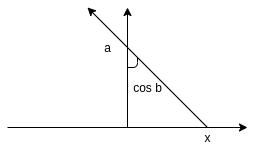
\includegraphics[scale=0.6]{images/universal_gravitation.png}
\end{center}
设$L$所在的直线为$x$轴,$y$轴过给定的单位质点. 由示意图这些力的合成一定是在$y$轴上的,关于$F_y$的微分为
$$
dF_y = k \frac{kdx}{a^2 + x^2} \cos b = \frac{kadx}{(a^2+k^2)^{\frac{3}{2}}}
$$
因此
$$
F_y = \int_{-\infty}^{+\infty} \frac{kadx}{(a^2+k^2)^{\frac{3}{2}}} = 2ka \int_{0}^{+\infty} \frac{dx}{(a^2+k^2)^{\frac{3}{2}}}
$$
令$x = a\tan u$,则有
$$
F_y = 2ka \int_{0}^{\frac{\pi}{2}} \frac{a\sec^2 u}{a^3\sec^3}du = \frac{2k}{a} \int_{0}^{\frac{\pi}{2}} \cos x dx = \frac{2k}{a}
$$
\end{example}

\subsection{待定参数}

\begin{example}
\rm 反常积分
$$
\int_0^{+\infty} \frac{1}{x^a(1+x)^b}dx
$$
收敛,求$a,b$.

\hints\ 这道题还是用柯西审敛法,注意要同时考虑积分上下限. 当$x \to +\infty$,那么就要和$\frac{1}{x^{\lambda}}(\lambda >1)$比较, 于是有
$$
\lim\limits_{x \to \infty} \frac{\frac{1}{x^a(1+x)^b}}{\frac{1}{x^{\lambda}}} = \frac{x^{\lambda-(a+b)}}{(\frac{1}{x}+1)^b},
$$
其中分母是趋于$0$,为保证分子不趋于无穷,则需要$\lambda < (a+b)$,即$a+b > 1$. 当$x \to 0$时,那么就要和$\frac{1}{x^{\lambda}}(\lambda < 1)$比较, 于是有
$$
\lim\limits_{x \to \infty} \frac{\frac{1}{x^a(1+x)^b}}{\frac{1}{x^{\lambda}}} = \frac{1}{x^{a-\lambda}(1+x)^b},
$$
其中$(1+x)^b \to 0$,则$a < \lambda$,即$a < 1$.
\end{example}

\subsection{分离积分}

\begin{example}
\rm 讨论下述积分的收敛性
$$
\int_0^{+\infty} \frac{\sin x}{x^2}dx  = \int_0^{\frac{\pi}{2}} \frac{\sin x}{x^2}dx + \int_{\frac{\pi}{2}}^{+\infty} \frac{\sin x}{x^2}dx
$$
\hints 其中后面这个积分在柯西判别法很容易确定是收敛的(实际上可以用狄利克雷判别法),因为总是满足
$$
f(x) \leq  \frac{1}{x^2}
$$
那么前面这个积分可以做一下变换
$$
\int_0^{\frac{\pi}{2}} \frac{\sin x}{x^2}dx =  \int_0^{\frac{\pi}{2}}  \frac{1}{x} \cdot \frac{\sin x}{x}dx \geq \frac{2}{\pi} \int_0^{\frac{\pi}{2}}  \frac{1}{x}
$$
这是因为$\frac{\sin x}{x}$在$(0,\frac{\pi}{2}]$上是单调减的,这一点求两次导即可知道,所以前面这个积分是发散的. 因此整个积分是发散的.  
\end{example}

\subsection{求值}

\begin{example}
\rm 求
$$
I = \int_0^{+\infty} \frac{dx}{1+x^4}.
$$
\hints\ \redt{方法1} 设$u = \frac{1}{x}$,则有
$$
I = \int_0^{+\infty} \frac{u^2}{1+u^4}du
$$
把这个积分和原积分加起来
$$
2I = \int_0^{+\infty} \frac{1+x^2}{1+x^4}dx = \int_0^{+\infty} \frac{1+\frac{1}{x^2}}{\frac{1}{x^2}+x^2}dx = \int_0^{+\infty} \frac{1+\frac{1}{x^2}}{(x-\frac{1}{x})^2+2}dx
$$
这里设$t = x-\frac{1}{x}$,有
$$
\int_{-\infty}^{+\infty} \frac{1}{t^2+2}dt = \left. \frac{1}{\sqrt{2}}\arctan \frac{t}{\sqrt{2}}\right|_{-\infty}
^{+\infty} = \frac{\pi}{\sqrt{2}}
$$
因此$I = \frac{\pi}{2\sqrt{2}}$. 

\redt{方法2} 可以考虑直接部分分式即,其中分母可以分解为
$$
1+x^4 = 1+2x^2+x^4 - 2x^2 = (1+x^2)^2 - 2x^2 = (x^2+\sqrt{2}x+1)(x^2-\sqrt{2}x+1).   
$$
因此
$$
\frac{1}{1+x^2} = \frac{Ax+B}{x^2+\sqrt{2}x+1} + \frac{Cx+D}{x^2-\sqrt{2}x+1} = \frac{\frac{1}{2\sqrt{2}}x+\frac{1}{2}}{x^2+\sqrt{2}x+1} + \frac{-\frac{1}{2\sqrt{2}}x+\frac{1}{2}}{x^2-\sqrt{2}x+1}
$$
即
$$
\frac{2\sqrt{2}}{1+x^2} = \frac{x+\sqrt{2}}{x^2+\sqrt{2}x+1} - \frac{x-\sqrt{2}}{x^2-\sqrt{2}x+1}
$$
原积分可以写作
$$
I = \frac{1}{2\sqrt{2}} \int_0^{+\infty} \frac{x+\sqrt{2}}{x^2+\sqrt{2}x+1} - \frac{x-\sqrt{2}}{x^2-\sqrt{2}x+1} dx = \frac{1}{2\sqrt{2}} \int_0^{+\infty} \frac{x+\sqrt{2}}{(x+\frac{\sqrt{2}}{2})^2+\frac{1}{2}} - \frac{x-\sqrt{2}}{(x-\frac{\sqrt{2}}{2})^2+\frac{1}{2}} dx
$$
再继续拆
$$
I = \frac{1}{2\sqrt{2}} \int_0^{+\infty} \frac{x+\frac{\sqrt{2}}{2}}{(x+\frac{\sqrt{2}}{2})^2+\frac{1}{2}} + \frac{\frac{\sqrt{2}}{2}}{(x+\frac{\sqrt{2}}{2})^2+\frac{1}{2}} - \frac{x-\frac{\sqrt{2}}{2}}{(x-\frac{\sqrt{2}}{2})^2+\frac{1}{2}} + \frac{\frac{\sqrt{2}}{2}}{(x-\frac{\sqrt{2}}{2})^2+\frac{1}{2}} dx
$$
第一项和第三项需要换元一下,令$u = x+\frac{\sqrt{2}}{2}$
$$
I = \frac{1}{2\sqrt{2}} \left[ \int_{\frac{\sqrt{2}}{2}}^{+\infty} \frac{u}{u^2+\frac{1}{2}}du  + \arctan \sqrt{2}\left.\left(x+\frac{\sqrt{2}}{2}\right)\right|_0^{+\infty}-\int_{-\frac{\sqrt{2}}{2}}^{+\infty} \frac{u}{u^2+\frac{1}{2}}du + \arctan \sqrt{2}\left.\left(x-\frac{\sqrt{2}}{2}\right)\right|_0^{+\infty}\right]
$$
其中
$$
\int_{\frac{\sqrt{2}}{2}}^{+\infty} \frac{u}{u^2+\frac{1}{2}}du - \int_{-\frac{\sqrt{2}}{2}}^{+\infty} \frac{u}{u^2+\frac{1}{2}}du =  - \int_{-\frac{\sqrt{2}}{2}}^{+\frac{\sqrt{2}}{2}} \frac{u}{u^2+\frac{1}{2}}du = 0. 
$$
因此
$$
I = \frac{1}{2\sqrt{2}}\left(\frac{\pi}{2}-\frac{\pi}{4} + \frac{\pi}{2}+\frac{\pi}{4}\right) = \frac{\pi}{2\sqrt{2}}
$$
\end{example}



\newpage
\section{微分方程}

\subsection{线性微分方程解的结构}

\begin{example}
\rm 已知$y_1 = e^{3x}-xe^{2x},y_2 = e^x - xe^{2x},y_3 = -xe^{2x}$是某二阶常系数非齐次线性微分方程的$3$个解,求该方程的通解.

\hints\ 这题考察线性微分方程解结构的一个非常典型的题,这里用到两个非齐次方程的解的差是齐次方程的解,则
$$
y_2  - y_3 = e^x , y_1 - y_3 = e^{3x}.
$$
它们是两个线性无关的解,因此它们是原方程导出的齐次方程的通解,我们再求一个特解即可,即$y_1-e^{3x} = -xe^{2x}$,则原方程的通解为
$$
y=C_1e^x + C_2e^{3x}-xe^{2x}. 
$$
\end{example}

\subsection{带积分的微分方程}

\begin{example}
\rm 设函数$f(x)$连续,且满足
$$
\int_0^x f(x-t)dt = \int_0^x (x-t)f(t)dt +e^{-x}-1
$$
求$f(x)$.

\hints\ 尝试去掉积分符号,去导前做一些变换,
$$
\begin{array}{rl}
\int_0^x f(u)du &= x\int_0^x f(t)dt - \int_0^x tf(t)dt + e^{-x}-1 \\
f(x) &= \int_0^x f(t)dt + xf(x)-xf(x)-e^{-x} \\
\end{array}
$$
\bluet{注意这里有$f(0)=-1$}(要善于发现这样的条件),设$y = \int_0^x f(t)dt$,于是
$$
y'-y = -e^{-x},
$$
根据一阶线性方程的通解我们有
$$
y = Ce^x + \frac{e^{-x}}{2},
$$
则$f(x) = Ce^x -\frac{e^{-x}}{2}$. 由于$f(0)=-1$,因此$C=-\frac{1}{2}$,最终$f(x)= -\frac{e^{x}+e^{-x}}{2}$. 
\end{example}

\newpage
\subsection{该死的绝对值}

\begin{annotation}
\rm 有时候的积分结果带$\ln|f(x)|$,这个时候在考虑要不要去绝对值的时候,可以采取的下述的手法
\begin{enumerate}
	\item 如果提供了某个点$(x_0,y_0)$,那么这个时候我们可以考虑去掉绝对值保留$x_0$所在的定义域,因为通解不需要表示全部的解,只要保证我们最终我们可以根据这个特殊的点确定某个特解即可!
	\item 如果没有提供某个点,那么这个时候我们可以有条件的去掉绝对值
	\begin{enumerate}
		\item 若是可分离变量方程,且里面没有无理数因子,我们可以把绝对值去掉
		\item 若是一阶线性方程,在对$P(x)$积分结果中出现$\ln|f(x)|$,根据$P(x)$中的是否有无理数因子或者分母为偶数的因子,如果有,那么这个绝对值不要去掉,最后分类讨论; 若没有,可以直接去绝对值. 
	\end{enumerate}
	\item 拿不准的时候,就彻底不去,直接开讨论就行. 
\end{enumerate}	
\end{annotation}

\begin{example}
\rm 求$y(1)=0$,且满足下述方程的$y$
$$
y'  = 1+\frac{y}{x} + \left( \frac{y}{x} \right)^2
$$
\hints\ 显然这个是一个齐次微分方程,令$u = \frac{y}{x}$,于是有
$$
\frac{du}{1+u^2} = \frac{dx}{x} \Rightarrow \arctan u = \ln |x|+C
$$
题目中已经给定了一个点$(1,0)$,那么此时我们可以去掉绝对值,只考虑$x > 0$的情况,即有
$$
u = \tan (\ln x + C) \Rightarrow y = x\tan (\ln x + C).
$$
最后带入特殊点,得到$C = 0$,最终有$y = x\tan (\ln x + C)$
\end{example}


\subsection{改变自变量}

\begin{example}
\rm 求下述方程的通解
$$
\frac{dy}{dx} = \frac{y}{x+y^4}
$$
\hints\ 当且形式根本找不到方法求,那么我们考虑求以$y$为自变量的$x=f(x)$形式的函数,于是有
$$
\frac{dx}{dy} = \frac{x+y^4}{y}  \Rightarrow \frac{dx}{dy} - \frac{x}{y} = y^3
$$
即是关于自变量$y$一个线性方程. 此时就可以直接用通项公式有
$$
x= y(\frac{1}{3}y^3 + C)
$$
\end{example}

\newpage
\section{解析几何}

\subsection{求直线在平面上的投影}

\begin{annotation}
\rm 如给定直线$L$和平面$S$,求$L$在$S$上投影直线方程. 
\begin{enumerate}
	\item 确定与$L$和$S$法向量$\eta$都垂直的向量$\gamma$; 、
	\item 确定以$\gamma$为法向量,包含$L$的平面$S'$;
	\item $S$和$S'$相交的直线就是$L$在$S$上的投影直线方程. 
\end{enumerate}
\end{annotation}


\subsection{旋转直线方程}

\begin{example}
\rm 求直线$L: \frac{x-3}{2} = \frac{y-1}{3} = z+1$绕直线$L_1: \left\{ \begin{array}{ll}
x = 2\\
y = 3 
\end{array}\right.$旋转一圈所产生的曲面方程.

\hints\ 这里要用一个低维的思想,我们任取$L$上一点$(x_0,y_0,z_0)$考察它绕直线$L_1$旋转得到的方程
$$
\left\{
\begin{array}{ll}
z = z_0 \\
(x-2)^2 + (y-3)^2 = (x_0-2)^2 + (y_0-3)^2
\end{array} \right.
$$
再考虑点$(x_0,y_0,z_0)$在直线$L$,目的是为了让上述方程取遍所有$L$上的点. 这里有
$$
\left \{
\begin{array}{ll}
x_0 = 2z_0 + 5\\
y_0 = 3z_0 + 4 
\end{array} \right.
$$
将它们带入第一个方程,即有
$$
(x-2)^2 + (y-3)^2 = (2z+3)^2 + (3z+1)^2,
$$
这就是我们要求的曲线方程. 
\end{example}

\newpage
\section{多元函数}

\subsection{带不等式的条件极值}

\begin{example}
\rm 求函数$z=f(x,y)=x^2-y^2 + 2$在椭圆域$D=\{(x,y)|x^2 + y^2 \leq 1\}$上的最大值和最小值. 

\hints\ 这个不等式的取值范围是一个闭连通域,我们只需要分别考虑它里面点构成的区域和边界上的点即可. 在这个椭圆里面唯一的驻点是$(0,0)$,其对应的函数值为$2$; 在椭圆上的点满足$y = 4 - 4^x$,则$f(x)$可以改写为
$$
z = x^2 - (4-4^x) +2 2 = 5x^2-2,
$$
其中$-1 \leq x \leq 1$,那么其最大值为$3$,最小值为$-2$. 三个驻点比较得出最终结果. 
\end{example}


\subsection{可微定义}

\begin{example}
\rm 设连续函数$z = f(x,y)$满足
$$
\lim\limits_{x \to 0 \atop y \to 1} \frac{f(x,y)-2x+y-2}{\sqrt{x^2 + (y-1)^2}} = 0,
$$
求$dz|_{(0,1)}$.

\hints\ 显然要从定义出发,目标是整理出来定义的形式,先求$f(0,1)$,由上式极限存在,可以得到
$$
\lim\limits_{x \to 0 \atop y \to 1} f(x,y) = 2x - y + 2,
$$
再由$f(x,y)$连续,上述等式左边就等于$f(0,1)$,等式右边是个有限极限,即$f(0,1)=1$. 我们再重新整理一下
$$
\lim\limits_{x \to 0 \atop y \to 1} \frac{f(x,y)-f(0,1)-2x+(y-1)}{\sqrt{x^2 + (y-1)^2}} = 0,
$$
这就是$f(x)$在点$(0,1)$处可微定义,即$dz|_{(0,1)} = 2dx - dy$. 
\end{example}

\newpage
\section{二重积分}



\subsection{交换次序更好积分}

\begin{example}
\rm 求积分
$$
\int_0^1 dy \int_y^1 \frac{\tan x}{x}dx.
$$
\hints\ 明显这个被积函数对$dx$是不好积的,于是考虑交换积分次序. 交换次序可以考虑画图来做,于是有
$$
\int_0^1 dx \int_0^x \frac{\tan x}{x} dy = \int_0^1 tan x dx = -\ln \cos x |_0^1  = - \ln \cos x.   
$$
\end{example}


\begin{example}
\rm 设$f(x)$为连续函数,定义
$$
F(x) = \int_1^x dv \int_v^x f(u)du , x > 1,
$$
求$F'(x)$.

\hints 二重积分求导,这显然直接求不了. 考虑先计算这个二重积分,现在的积分次序导致我们无法对$\int f(u)du$处理,所以先交换次序. 有
$$
F(x) = \int_1^x du \int_1^u f(u)dv = \int_1^x (u-1)f(u)du.
$$
被积函数是连续函数的变上限积分,它的导数为$(x-1)f(x)$. 
\end{example}

\subsection{化极坐标}

\begin{example}
\rm 求积分
$$
\int_0^2 dx \int_0^{\sqrt{2x-x^2}} \sqrt{x^2+y^2}dy.
$$
\hints\ 被积函数出现$x^2 + y^2$,考虑化极坐标. 首先把极坐标方程写出来,确定$\theta$变限在$[0,\frac{\pi}{2}]$,当固定一点$x$时,此时$0 \leq y \leq \sqrt{2x-x^2}$,那么考虑这个积分域的边界就有
$$
x^2 + y^2 = \rho^2 = 2\rho\cos \theta \Rightarrow \rho = 2\cos\theta.
$$
于是原积分为
$$
\int_0^{\frac{\pi}{2}}d\theta \int_0^{2\cos\theta}\rho^2 d\rho = \int_0^{\frac{\pi}{2}} \frac{8\cos^3\theta}{3} d\theta = \frac{8}{3}\int_0^{\frac{\pi}{2}} (1-\sin^2\theta)d\sin\theta  = \frac{8}{3}(\sin\theta-\frac{\sin^3\theta}{3})\big|_0^{\frac{\pi}{2}} = \frac{16}{9}.
$$
\end{example}

\newpage
\section{三重积分}

\subsection{直角坐标}

\begin{example}
\rm 设$\Omega$由$x^2 + \frac{y^2}{2^2} + \frac{z^2}{3^2} \leq 1, 0 \leq z \leq 1$所确定,求
$$
\iiint\limits_{\Omega} z^2dv
$$

\hints\ 显然这是一个椭圆区域,因此先考虑二重积分再单重积分,$xOy$上椭圆方程为
$$
\frac{x^2}{1-\frac{z^2}{3}} + \frac{y^2}{2^2(1-\frac{z^2}{3})} = 1
$$
这里可以直接套公式得出该椭圆面积为$S=\pi ab= 2\pi(1-\frac{z^2}{3})$. 因此
$$
\iiint\limits_{\Omega} z^2dv = 2\pi \int_0^1 z^2(1-\frac{z^2}{3})dz = \frac{28}{45}\pi
$$
\end{example}


\begin{example}
\rm 设$\Omega$是由曲面$z = x^2+y^2, y=x, y=0, z=1$在第一卦限所围成的区域,$f(x,y,z)$在$\Omega$上连续,求$\iiint_\Omega f(x,y,z)dv$直角坐标表示$\int dy \int dx \int f(x,y,z)dz$. 

\hints\ 先是在$xOy$上积分,那么先确定$\Omega$在其上的投影. 确定几条平面曲线: (1 因为$z=1$,那么椭圆抛物面在$xOy$上投影为$x^2+y^2 = 1$. (2 $y=x$ (3 $y=0$ (4 第一象限. 借助前面这些条件$xOy$上的投影是可以确定了. 对$z$积分,可以想象我们在平面上对抛物线积分. 
\end{example}

\subsection{柱坐标}

\subsection{球坐标}


\newpage
\section{多元积分的应用}

\subsection{第一类曲线积分}

\begin{annotation}
\rm 第一类曲线积分的一般解决方法:
\begin{enumerate}
	\item 确定是平面曲线还是空间曲线;
	\item 确定曲线方程的给定形式和自变量的变换范围, 注意无论怎样的曲线方程都是可以看做参数方程的;
	\item 确定是否为特殊曲线做简化计算的操作,例如关于坐标轴的对称,轮换对称性等;
	\item 若是曲线积分化定积分. 这一过程要注意弧长微分替换积分变量的过程,而提到的参数方程的弧长微分为$\sqrt{x(t)'^2 + y(t)'^2 + z(t)'^2}dt$.  
\end{enumerate}
\end{annotation}

\subsection{第二类曲线积分}

\begin{annotation}
\rm 第二类曲线积分的一般解决方法:
\begin{enumerate}
	\item 确定是平面曲线还是空间曲线;
	\item 确定曲线方向;
	\item 确定曲线方程的给定形式和自变量的变换范围, 注意无论怎样的曲线方程都是可以看做参数方程的;
	\item 确定\redt{平面曲线}积分是否与路径无关,常见判定手法(1 $Pdx+Qdy$是否是某个二元函数的全微分 (2 $\frac{\partial P}{\partial y} = \frac{\partial Q}{\partial x}$. 若与路径无关考虑, (1 利用原函数直接计算 (2 化简单积分路线,例如平行于坐标轴,就化为两个定积分. 
	\item 确定是否为光滑的\redt{平面闭曲线},若为光滑曲线考虑使用格林公式化二重积分,注意曲线方向和其围成的区域$D$要遵守左手法则,即绕着曲线的方向绕一圈,区域$D$总是在观察者的左手边. 还需要注意被积函数$P,Q$在$D$上要有连续的一阶偏导;
	\item 确定若不是\redt{平面闭曲线},可以考虑做补线让其变成一个闭曲线,再使用格林公式,可能可以简化计算. 
	\item 确定是否为\redt{空间闭曲线},若是空间闭曲线,考虑使用斯托克斯公式,注意曲线方向和曲面的法向量要遵守右手法则. 
	$$
	\int_L P(x,y,z)dx + Q(x,y,z)dy + R(x,y,z)dz = \int\int_\sum (\frac{\partial R}{\partial y}-\frac{\partial Q}{\partial z})dydz + (\frac{\partial P}{\partial z}-\frac{\partial R}{\partial x})dzdx + (\frac{\partial Q}{\partial x}-\frac{\partial P}{\partial y})dxdy
	$$
	\item 直接计算,使用公式
	$$
	\int_L P(x,y,z)dx + Q(x,y,z)dy + R(x,y,z)dz = \int_\alpha^{\beta} P[x(t),y(t),z(t)]x'(t) + Q[x(t),y(t),z(t)]y'(t) + R[x(t),y(t),z(t)]z'(t)dt.
	$$ 
\end{enumerate}
\end{annotation}

\subsection{两类曲线积分关系}

\begin{example}
\rm 设$L$是圆周$x^2 + y^2 = 1$,$\bm{n}$为$L$的外法线向量,$u(x,y) = \frac{1}{12}(x^4 + y^4)$,求
$$
\oint_L \frac{\partial u}{\partial \bm{n}}ds.
$$
\hints\ 由方向梯度有
$$
\frac{\partial u}{\partial \bm{n}} = \frac{\partial u}{\partial x}\cos\alpha + \frac{\partial u}{\partial y}\cos \beta,
$$
其中$\cos\alpha,\cos\beta$分别是$\bm{n}$方向余弦. 这里有两种手法来尝试计算.  

\bluet{方法1} 先展开这个方向导数
$$
\frac{\partial u}{\partial \bm{n}} = \frac{1}{3}x^3\cos\alpha + \frac{1}{3}y^3\cos\beta,
$$
这里我们尝试把$\cos\alpha$和$\cos\beta$求出来. 将对$L$曲线积分变成在极坐标下的普通积分,
$$
\left\{
\begin{array}{ll}
x = \cos\theta \\
y = \sin\theta
\end{array}\right.
$$
其上任意一点$(\cos \theta,\sin\theta)$处的外法线向量为
$$
\bm{n} = (\cos\theta, \sin\theta),
$$
因此
$$
\cos\alpha = \frac{\cos\theta}{\sqrt{{\cos\theta^2 + \sin^2\theta}}}, \cos\beta =\frac{\sin\theta}{\sqrt{{\cos\theta^2 + \sin^2\theta}}},
$$
最终积分变为
$$
I = \int_{0}^{2\pi} \frac{\cos^4\theta + \sin^4\theta}{3}d\theta = \frac{\pi}{2}
$$
\bluet{方法2} 这里用到第一类曲线积分和第二类曲线积分的联系. 设$L$上任意一点$(x,y)$处的逆时针方向切线$l$与$x,y$轴的方向余弦分别为$\cos\gamma,\cos\delta$. 那么这个$\bm{n}$相当于是$l$顺时针旋转$\frac{\pi}{2}$得到的,于是
$$
\cos\alpha = \cos\delta, \cos\beta = -\cos\gamma.
$$
因此原积分变为
$$
\begin{aligned}
I  &= \oint_L \frac{\partial u}{\partial x}\cos\delta -\frac{\partial u}{\partial y}\cos\gamma ds \\
&= \oint_L\frac{\partial u}{\partial x}dy -\frac{\partial u}{\partial y}dx & \text{(两类积分的转换)} \\
&= \iint\limits_{x^2 + y^2 \leq 1} \frac{\partial^2 u}{\partial x^2} + \frac{\partial^2 u}{\partial y^2}d\sigma & \text{(格林公式)} \\
&= \int_{0}^{2\pi}d\theta \int_0^1 \rho^3dp \\
&= \frac{\pi}{2}
\end{aligned}
$$

\end{example}

\subsection{第一类曲面积分}

\begin{annotation}
\rm 第一类曲面积分的一般计算方法
\begin{enumerate}
	\item 确定曲面方程,实际上只有一种$z=f(x,y)$,并没有复杂的参数方程,和其自变量变化范围; 
	\item 确定是否为特殊的曲面做简化计算,例如关于坐标轴平面对称,轮换对称性等;
	\item 直接计算,使用曲面微分的变量替换,需要注意$x,y$的区域$D$的确定
	$$
\int\int_\sum f(x,y,z)dS = \int\int_D\sqrt{1+f_x^2(x,y),f_y^2(x,y)}dxdy.
$$
\end{enumerate}
\end{annotation}

\begin{example}
\rm 设$\Sigma$为球面$x^2 + y^2 + z^2 = 2ax$,求曲面积分
$$
I =\iint_{\Sigma} (x^2 + y^2 + z^2)dS.
$$

\hints\ 这道理按照球面来积分,好像有点难受. 首先我们做一个简单的代换
$$
I = \iint_{\Sigma} 2ax dS = 2a \iint_{\Sigma} xdS,
$$
其中$\iint_{\Sigma} xdS$可以看求曲面形心的$\bar{x}$中的分子,且球面的形心的$\bar{x} = a$,从而
$$
I = 2a \cdot a \cdot 4\pi a^2 = 8\pi a^4. 
$$
\end{example}

\subsection{第二类曲面积分}

\begin{annotation}
\rm 第二类曲面积分的一般计算方法
\begin{enumerate}
	\item 确定曲面方程,实际上只有一种$z=f(x,y)$,并没有复杂的参数方程,和其自变量变化范围; 
	\item 确定曲面的方向;
	\item 确定曲面是否可以围成一个闭区域,考虑使用高斯公式
	$$
	\int\int_\sum Pdydz + Qdzdx + Rdxdy = \int\int\int_\Omega (\frac{\partial P}{\partial x}+\frac{\partial Q}{\partial y}+\frac{\partial R}{\partial z})dv.
	$$
	这里曲面需要取外侧方向,如果当且曲面是内侧方向则需要加负号,也需要确定$P,Q,R$是否具有一阶连续偏导. 
	\item 考虑是否可以增加补面围成一个闭区间来使用高斯公式. 
	\item 直接计算,上述给定是$z$关于$x,y$方程,那么曲线方向决定了曲面法线和$z$轴的夹角余弦值,若余弦值是负的,则需要在下式积分号就带负号
	$$
	\int\int_{S} f(x,y,z)dxdy = \pm \int\int_{D_{xy}} f(x,y,f(x,y))dxdy.
	$$
	这里要注意若给定是$y$关于$x,z$的方程,这里的余弦值则是看曲面法向量和$y$轴的夹角. 
\end{enumerate}
\end{annotation}

\newpage
\section{级数}

\subsection{级数判定总结}

\begin{annotation}
\rm 一些有用的资料
\begin{enumerate}
	\item \href{https://sites.lafayette.edu/thompsmc/files/2016/03/Series_Summary.pdf}{遇到一个级数应该用怎样的手法总结}.
	\item \href{https://en.wikipedia.org/wiki/Convergence_tests}{级数判定手法大全}.
\end{enumerate}
\end{annotation}

\subsection{极限test}

\begin{example}
\rm 讨论下述级数的收敛性
$$
\sum\limits_{n=1}^\infty (n\ln\frac{2n+1}{2n-1} -1). 
$$

\hints\ 这里很难拿哪一个级数来做极限test,观察$n\ln t$,我们可以将其泰勒展开,找到最小的无穷小. 于是
$$
\ln(1+\frac{2}{2n-1}) = \frac{2}{2n-1} - \frac{1}{2}(\frac{2}{2n-1})^2 +  \frac{1}{3}(\frac{2}{2n-1})^2 + o((\frac{2}{2n-1})^3). 
$$
那么
$$
\begin{array}{ll}
n\ln(1+\frac{2}{2n-1}) - 1 &= -1 + \frac{2n}{2n-1} - \frac{n}{2}(\frac{2}{2n-1})^2 +  \frac{n}{3}(\frac{2}{2n-1})^2 + o(n(\frac{2}{2n-1})^3) \\
&= \frac{2n+3}{3(2n-1)}(\frac{1}{2n-1})^2 + o(\frac{8n}{(2n-1)}(\frac{1}{2n-1})^2)
\end{array}
$$
因此
$$
\lim\limits_{n \to \infty} \frac{n\ln\frac{2n+1}{2n-1} -1}{(\frac{1}{2n-1})^2} = \frac{1}{3},
$$
其中级数$\sum\limits_{n \to \infty}(\frac{1}{2n-1})^2$是收敛的,所以原级数也是收敛的. 
\end{example} 

\subsection{参数收敛}
\begin{example}
\rm 讨论下列级数收敛性
$$
\sum\limits_{n=1}^{\infty} \frac{\ln (n!)}{n^\alpha}
$$
\hints\ 展开$\ln n!$,有
$$
\ln n! = \ln 1 + \ln 2 + \cdots \ln n < n\ln n < n^{1+\beta},
$$
在$n$足够大的时候,对任何$\beta > 0$都是成立. 因此
$$
\frac{\ln (n!)}{n^\alpha} < \frac{n^{1+\beta}}{n^\alpha} = n^{1+\beta - \alpha},
$$
因此取$\alpha > 2$时,存在$\beta$使得
$$
\frac{\ln (n!)}{n^\alpha} < \frac{1}{n} < \frac{n^{1+\beta}}{n^\alpha}. 
$$
即原级数在$a > 2$是收敛的. 同理若$\alpha \leq 2$时,是存在$\beta$使得$1+\beta-\alpha > -1$的,此时是无法判定其是否收敛的。 
\end{example}

\begin{example}
\rm 已知级数$\sum\limits_{n=1}^{\infty} \frac{\sqrt{n+1}}{n^\alpha}$收敛,求$\alpha$取值. 

\hints\ 先用比较审敛法确定一收敛与原级数收敛性相同的级数,显然这样选择一个调和级数$\frac{1}{n^{\alpha-\frac{1}{2}}}$,来验证一下
$$
\lim\limits_{n \to \infty} \frac{\frac{\sqrt{n+1}}{n^\alpha}}{\frac{1}{n^{\alpha-\frac{1}{2}}}} = \lim\limits_{n \to \infty} \sqrt{\frac{n+1}{n}} = 1.
$$
判定调和级数的收敛性,需要$\alpha > \frac{3}{2}$. 
\end{example}

\subsection{带-1的幂次}
\begin{example}
\rm 判断下述级数的收敛性
$$
\sum\limits_{n=2}^{\infty}\frac{1+(-1)^n}{\ln n}
$$
\hints\ 这个级数奇数时为零,因此我们写作
$$
\sum\limits_{n=1}^{\infty}\frac{2}{\ln 2n}
$$
这个级数显然是发散的,因为在$n$足够大时$\frac{2}{\ln 2n} \geq \frac{1}{n}$.
\end{example}

\subsection{不标准的幂级数}
\begin{example}
\rm 求幂级数
$$
\sum\limits_{n=1}^\infty \frac{n}{2^n + (-3)^n}x^{2n-1}
$$
的收敛半径. 

\hints 这是一个不标准的幂级数,无法直接用结论. 所以先化标准的形式$a_nx^n$. 先考虑积分,消掉指数的常数,即有
$$
\sum\limits_{n=1}^\infty \int_0^{x} \frac{n}{2^n + (-3)^n}x^{2n-1} = \sum\limits_{n=1}^\infty \frac{1}{2(2^n + (-3)^n)}x^{2n}.
$$
再令$u = x^2$,求$ \sum\limits_{n=1}^\infty \frac{1}{2(2^n + (-3)^n)}u^{n}$的收敛半径,根据结论有
$$
\lim\limits_{n \to \infty} \left| \frac{2^n+(-3)^n}{2^{n+1}+(-3)^{n+1}}\right| = \frac{1}{3},
$$
因此其收敛半径为$3$,所以$|x| <\sqrt{3}$,即原级数的收敛半径为$\sqrt{3}$. 
\end{example}

\subsection{利用傅里叶公式求和}

\begin{example}
\rm 求下列级数的和
$$
\sum\limits_{n = 1}^{+\infty} \frac{(-1)^n \sin n}{n}
$$
\hints\ 考虑$s(x) = \frac{x}{\pi}$在$(-\pi,pi)$上的傅里叶级数,它是一个奇函数因此
$$
s(x) = \sum\limits_{n=1}^{+\infty} b_n \sin nx = \sum\limits_{n=1}^{+\infty} \left(\frac{2}{\pi}\int_{0}^{\pi} \frac{x}{\pi} \sin nx dx  \sin nx \right) =  \sum\limits_{n=1}^{+\infty} -\frac{2}{\pi}\frac{(-1)^{n}\sin nx}{n}.
$$
显然有
$$
s(1) = -\frac{2}{\pi} \sum\limits_{n = 1}^{+\infty} \frac{(-1)^n \sin n}{n} = \frac{1}{\pi},
$$
因此$\sum\limits_{n = 1}^{+\infty} \frac{(-1)^n \sin n}{n} = -\frac{1}{2}$. 
\end{example}


\subsection{利用已有的幂级数求和}

\begin{example}
\rm 求下述幂级数的和函数
$$
\sum\limits_{n=1}^{\infty} (-1)^n \frac{2n+1}{(2n)!}x^{2n}.
$$

\hints\ 这个级数显然不能在有限次的积分或者求导来一般手法求和,考虑把它拆开成熟悉的级数,这里可以拆成两个熟悉的三角函数:
$$
S(x) = \sum\limits_{n=1}^{\infty}(-1)^n \frac{1}{(2n-1)!}x^{2n-1}x + \sum\limits_{n=0}^{\infty} (-1)^n \frac{1}{(2n)!}x^{2n}-1 = -x\sin x + \cos x -1. 
$$

\end{example}

\subsection{构造微分方程}

\begin{example}
\rm 求下述幂级数的和函数
$$
\sum\limits_{n=0}^{\infty} (-1)^n \frac{x^{2n}}{(2n)!!}
$$
\hints\ 连续的求导和积分似乎很难做到,这里就很有技巧了,可以构造含$S(x)$一阶微分方程. 其中
$$
S'(x) = \sum\limits_{n=1}^{\infty} (-1)^n \frac{x^{2n-1}}{(2n-2)!!} = \sum\limits_{n=1}^{\infty} (-1)^n \frac{x^{2n-2} x}{(2n-2)!!} = -xS(x),
$$
解这个微分方程得到$S(x)= Ce^{-\frac{1}{2}}$,因为这里$S(0)=1$,最终得到$S(x) = e^{-\frac{1}{2}x^2}$. 
\end{example}

\subsection{化增量公式}

\begin{example}
\rm 求下述幂级数的和函数
$$
\sum\limits_{n=0}^{\infty} \frac{x^{2n+1}}{(2n+1)!}
$$

\hints\ 观察这个系数有点像$e^x$的幂级数,但是只有奇数项. 那么偶数项其实就是$S'(x)$,因此$S'(x) +S(x) = e^x$,由此解得$S(x)= Ce^{-x} + \frac{1}{2}e^{x}$,由$S(0) = 0$,最终可得$S(x) = -\frac{1}{2}e^{-x} + \frac{1}{2}e^{x}$
\end{example}


\begin{example}
\rm 考虑调和级数$\sum\limits_{n=1}^{\infty} \frac{1}{n}$的收敛性.

\hints\ 这次我们不从部分和出发,我们考虑它和另级一个发散的级数
$$
\sum\limits_{n=1}^{\infty} [\ln(n+1) - \ln n],
$$
来比较. 考虑这个函数$\ln(n+1) - \ln n$在$[n,n+1]$上的增量公式
$$
\ln(n+1) - \ln n = \frac{1}{(n+\theta)}, \theta
$$
于是
$$
\frac{1}{(n+\theta)} < \frac{1}{n}, 
$$
因此$\frac{1}{n}$是收敛的. 
\end{example}

\begin{example}
\rm 考虑级数$\sum\limits_{n=0}^{\infty} \frac{x^{2n+1}}{(2n+1)!} \frac{1}{n^{1+s}}$的收敛性,其中$s > 0$. 

\hints 同样引入收敛级数$\sum\limits_{n=0}^{\infty} \frac{1}{(n-1)^s} - \frac{1}{(n)^s}$来做比较. 考虑函数$\frac{1}{(n-1)^s} - \frac{1}{(n)^s}$在$[n-1,n]$上的增量公式
$$
\frac{1}{(n-1)^s} - \frac{1}{(n)^s} = \frac{1}{(n-\theta)^{1+s}}, 0 < \theta < 1,
$$
那么
$$
\frac{1}{n^{1+s}} < \frac{1}{(n-\theta)^{1+s}},
$$
因此原级数收敛. 
\end{example}

\begin{example}
\rm 分析下述级数的收敛性
$$
\sum\limits_{n=2}^{\infty} \frac{1}{n\ln n}. 
$$
\hints\ 那个级数要比调和级数每一项$\frac{1}{n}$小那么一点,因此考虑和$\frac{1}{n^s}$比较,也可以换个级数来比较. 考虑级数
$$
\sum\limits_{n=2}^{\infty} \ln\ln(n+1) - \ln\ln n, 
$$
显然这级数是发散的,如果我们考虑函数$\ln\ln(n+1) - \ln\ln n$在$[n,n+1]$上的增量公式
$$
\ln\ln(n+1) - \ln\ln n = \frac{1}{(n+\theta)\ln(n + \theta)}, 0 < \theta < 1,
$$
那么有
$$
\frac{1}{(n+\theta)\ln(n + \theta)} < \frac{1}{n\ln n},
$$
因此原级数发散. 
\end{example}

\newpage
\section{tricks}

\subsection{一些有趣的不等式}

\begin{proposition}\label{prop: bonuli}
$$
a^{\frac{1}{n}}-1 < \frac{a-1}{n},\; a > 1.
$$
\hints\ {\color{red}伯努利不等式}.
$$
(1+x)^n \leq 1 + nx, \; n \geq 0, x \leq -1.
$$
使得$(1+x) = a^{\frac{1}{n}}$,即可得到上式.
\end{proposition}

\begin{proposition}
\rm 
$$
\sin x < x , 0 < x < +\infty
$$
\end{proposition}

\begin{proposition}
\rm 
$$
\ln(1+x) < x,  -1< x < +\infty
$$
\end{proposition}

\subsection{Stirling公式}

\begin{proposition}
\rm 
$$
\ln(n!) = n\ln n-n+O(\ln n). 
$$
\bluet{经常用于拆解$\ln n!$有奇效}. 
\end{proposition}


\subsection{高数积分}

\begin{proposition}
\rm 
$$
\int _{-\infty }^{\infty }e^{-\alpha x^{2}}\,dx={\sqrt {\frac {\pi }{\alpha }}}
$$
\end{proposition}

\end{document}